\documentclass[tikz,border=2pt]{standalone}
\usepackage{amsmath,amssymb}
\usepackage{pgfplots}
\pgfplotsset{compat=1.18}

\begin{document}
% A discrete random variable takes finitely (or countably) many values, each with a definite
% probability: X = number of heads in two fair tosses has pmf 1/4, 1/2, 1/4 on 0, 1, 2.
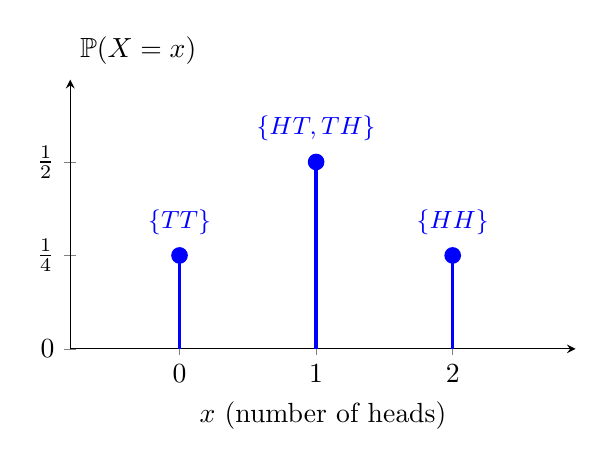
\begin{tikzpicture}
	\begin{axis}[
		axis lines=left, xmin=-0.8, xmax=2.9, ymin=0, ymax=0.72,
		xtick={0,1,2}, ytick={0,0.25,0.5}, yticklabels={$0$,$\tfrac14$,$\tfrac12$},
		xlabel={$x$ (number of heads)}, ylabel={$\mathbb{P}(X=x)$}, ylabel style={rotate=-90, anchor=south west, at={(axis description cs:0,1.02)}},
		width=8cm, height=5cm, clip=false
		]
		\addplot[ycomb, blue, very thick, mark=*, mark size=2.4pt] coordinates {(0,0.25) (1,0.5) (2,0.25)};
		\node[blue, anchor=south, font=\small] at (axis cs:0,0.28) {$\{TT\}$};
		\node[blue, anchor=south, font=\small] at (axis cs:1,0.53) {$\{HT,TH\}$};
		\node[blue, anchor=south, font=\small] at (axis cs:2,0.28) {$\{HH\}$};
	\end{axis}
	
\end{tikzpicture}
\end{document}
